%
\section{Metodi di Machine Learning}
\label{sec:metodi di machine learning}
%

In questa sezione verranno presentate, in maniera descrittiva, le più popolari metodologie di machine learning.\\

\subsection{Iperparametri e Grid Search}
\label{iperparametri e grid search}

Prima di parlare del Grid Search è necessario introdurre il concetto di \textbf{iperparametro}. Come detto nelle sezioni precedenti, un modello di apprendimento è caratterizzato da una serie di parametri che vengono modificati in maniera iterativa in modo da minimizzare la Loss function e, come noto, tale processo avviene attraverso un continuo confronto con il training data set. Quando si parla di iperparametri si intende invece una serie di parametri che caratterizzano il modello implementato che non sono modificati nel processo di addestramento con il training data set ma vengono prestabiliti dall'utente. \\
Chiaramente al variare degli iperparametri cambia anche la qualità del processo di apprendimento del modello e quindi anch'essi devono essere sottoposti ad un processo di ottimizzazione. A questo punto entra in gioco il metodo del Grid Search che è appunto un metodo di ottimizzazione degli iperparametri. \\
Il Grid Search è piuttosto semplice sia da comprendere concettualmente sia da implementare nella pratica; fa parte dei così detti "Brute-Force Search", cioè di quei metodi che si basano sulla sistematica verifica di tutte le possibili soluzioni ad un problema per poi considerare la migliore. Per esempio si consideri il problema di dover cercare i divisori di un numero n: un approccio "Brute-Force" prevedrebbe di considerare tutti i numeri minori di n e verificare quelli per i quali la divisione non dà resto. Questo esempio permette anche di mettere in evidenza il limite principale di tale tipologia di approccio: il numero di possibilità da esplorare può aumentare molto velocemente, soprattutto se si considera un processo multivariato. \\
Tornando ora nello specifico al Grid Search, si consideri un modello caratterizzato da un numero k di iperparametri. Si può definire, in analogia a ciò che è stato fatto con i parametri, un vettore le cui componenti sono appunto gli iperparametri: 
\begin{equation}
\bm{\mu} = (\mu_1,...,\mu_k)
\end{equation}
Tale vettore apparterrà ovviamente ad uno spazio k-dimensionale, sul quale può essere costruita una griglia i cui nodi corrispondono a particolari combinazioni degli iperparametri. \\
A questo punto si può avviare l'apprendimento del modello per ogni particolare configurazione degli iperparametri ed ottenere un valore per la Loss function. Si arriva allora ad avere una valore della Loss per ogni nodo della griglia e quindi basta considerare quello per il quale la Loss è minore, ottenendo la miglior configurazione degli iperparametri. \\
In Figura ~\ref{fig:Grid Search} nella pagina seguente è riportato per chiarezza un esempio visivo dell'esito di un processo di ottimizzazione degli iperparametri attraverso il metodo Grid Search.

\begin{figure}[h!]
	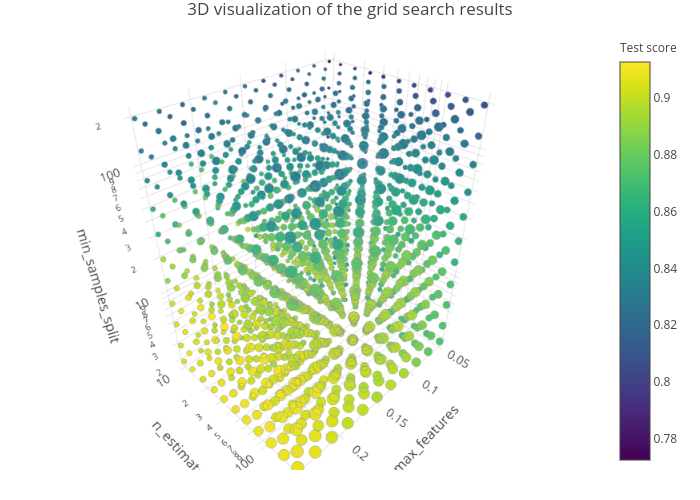
\includegraphics[width=\linewidth]{figs/Grid_immagine.png}
	\caption{la figura illustra visivamente l'esito di un processo di ottimizzazione degli iperparametri attraverso il metodo Grid Search (~\cite{knuthwebsite})}
	\label{fig:Grid Search}
\end{figure}
\newpage 

Come accennato precedentemente, man mano che aumenta la complessità del modello è molto probabile che aumenti il numero degli iperparametri e quindi la dimensionalità dello spazio introdotto precedentemente; ciò implica l'aumento considerevole del numero di configurazioni degli iperparametri da esplorare attraverso il Grid Search e quindi il tempo necessario per concludere l'ottimizzazione.\\
E' possibile ovviare parzialmente a questo problema attraverso il Random Grid Search (RGS), dove non sono considerati tutti i nodi della griglia, ma solo una loro parte selezionata in maniera casuale secondo una particolare distribuzione (ciò permette anche di tener conto di conoscenze pregresse). \\
Come esempio si riporta un problema molto comune nel campo della fisica delle alte energie, ovvero la separazione del segnale dal fondo. Si consideri, per semplicità, un processo bi-variato $\textbf{x} = (x_1,x_2)$ dove, per raggiungere l'obiettivo prefissato di separazione fra segnale e fondo, è necessario applicare un così detto taglio, ovvero stabilire un punto nello spazio bidimensionale $\textbf{P} = (P_1,P_2)$ che permette di dividere lo stesso in due porzioni, come illustrato in Figura ~\ref{fig:grid_example}.\\
Chiaramente la scelta di tale punto deve essere fatta in modo da ottimizzare la separazione segnale-fondo e quindi si può utilizzare il metodo del Grid Search o meglio il RGS per le ragioni presentate precedentemente. 

\begin{figure}[h!]
	\centering
	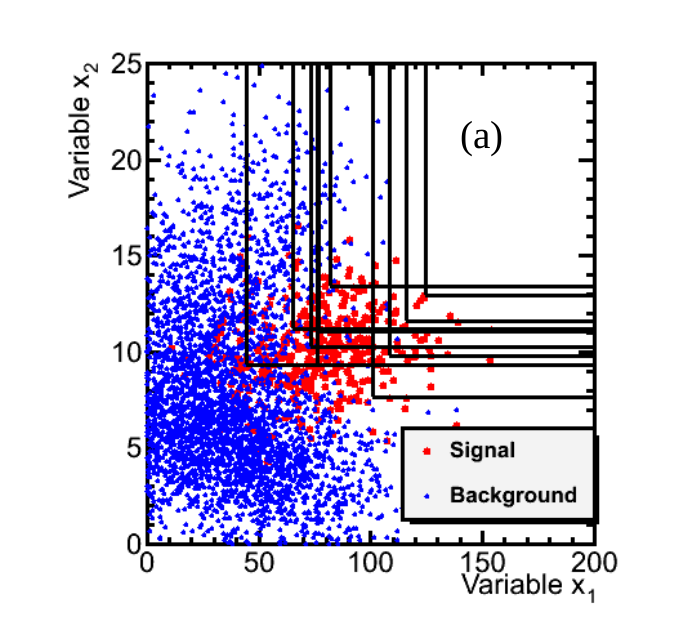
\includegraphics[width=0.85\textwidth]{figs/Grid_example.png}
	\caption{risultato grafico di un processo di Random Grid Search per la separazione del segnale dal fondo in un processo bi-variato. L'immagine è presa da \cite{Metodi_multivariati}.}
	\label{fig:grid_example}
\end{figure}
\newpage

Come si evince dalla figura, un notevole limite del Grid search in questo caso particolare (e della sua variante RDG) sta nell'essere vincolati a dei tagli paralleli agli assi e quindi ci si trova difronte ad un risultato piuttosto limitante. Si possono introdurre a questo punto i Metodi Lineari, continuando a seguire il percorso già accennato in precedenza, ovvero partire dal metodo concettualmente e praticamente più semplice ma meno efficiente per poi salire mano mano di complessità e di efficienza.\\

\newpage

\subsection{Analisi discriminante lineare}
\label{metodi lineari e discriminante di Fisher}

Come detto nella sezione precedente, il GS ed il RDG possono essere utilizzati per la separazione del segnale dal fondo ma hanno dei limiti piuttosto considerevoli che sono già stati illustrati. L'analisi discriminante è un metodo che permette di raggiungere lo stesso obiettivo di separazione, ma in modo più efficiente. \\
L'analisi discriminante si definisce lineare quando la funzione classificatrice è, appunto, lineare. \\
Si immagini di avere a disposizione un determinato set di eventi in input $\textbf{x}_\textbf{i}$, ciascuno caratterizzato da un numero n di variabili (spazio n-dimensionale) e di volerli ripartire fra segnale e fondo.\\
Si definisce la funzione discriminante lineare nel seguente modo:
\begin{equation}
D(x_1 , x_2 , ... , x_n) = c_0 + c_1x_1 + ... +c_nx_n = c_0 + \sum_{i=0}^{n} c_ix_i 
\end{equation}
quindi come una combinazione lineare delle componenti del vettore che rappresenta l'evento; il valore assunto dalla funzione per ogni singolo evento ne permette la separazione nelle due classi (nel presente caso segnale e fondo), utilizzando un valore di riferimento $D_0$. \\
A questo punto l'obiettivo è quello di massimizzare la distanza fra le due classi, ovvero rendere massima la differenza dei valori assunti dalla funzione $D(\textbf{x})$ fra gli eventi appartenenti al fondo e quelli relativi al segnale. \\
Un esempio di questo approccio è il metodo proposto da Fisher: si consideri un campione di eventi appartenenti al segnale e se ne definisca la media $\bm\mu_\textbf{s}$ e la deviazione standard $\sigma_s$ ed un campione appartenente al fondo, definendo anche qui la media $\bm\mu_\textbf{f}$ e la deviazione standard $\sigma_f$. A questo punto la migliore configurazione dei parametri è quella che massimizza la seguente funzione: 
\begin{equation}
F(\textbf{c}) = \frac{(\bm\mu_\textbf{s} - \bm\mu_\textbf{f})^2}{\sigma_s^2 + \sigma_f^2}
\end{equation} 
\newpage

\subsection{Reti Neurali}
\label{reti neurali}
La struttura di una rete neurale prevede la presenza di unità fondamentali, dette neuroni, che sono organizzate in strati e legate fra di loro mediante delle connessioni (sinapsi), ciascuna delle quali è caratterizzata da un peso. Sono proprio questi pesi a giocare un ruolo fondamentale nel processo di apprendimento della rete perché sono loro i parametri soggetti a modifica.\\
Il nome rete neurale (artificiale) deriva dal fatto che la loro struttura è inspirata dalle corrispondenti strutture biologiche (seppur di molto semplificata). \\
In una rete neurale è sempre presente uno strato di input ed uno di output, mentre il numero di livelli nascosti può variare a seconda della complessità della rete; In figura ~\ref{fig:schemaNN} è riportato un esempio di rete neurale con un singolo strato interno nascosto.
\begin{figure}[h!]
	\centering
	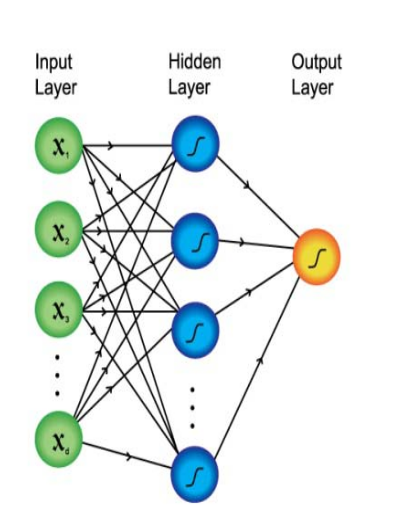
\includegraphics[width=0.50\textwidth]{figs/schemaNN.png}
	\caption{si riporta un esempio grafico di rete neurale formata da un unico strato nascosto. L'immagine è presa da \cite{Metodi_multivariati}.}
	\label{fig:schemaNN}
\end{figure}
\\
Si può passare ora a presentare il modello del singolo neurone per capire com'è strutturato e quale compito svolge.
Gli elementi che caratterizzano il singolo neurone sono:
\begin{enumerate}
	\item Una serie di connessioni in ingresso (ciascuna caratterizzata da un proprio peso);
	\item Un sommatore che ha il compito di svolgere la somma pesata degli input, utilizzando i pesi caratteristici delle connessioni;
	\item Un output e la relativa funzione di attivazione, che viene usata per limitarne l'ampiezza (tipicamente ad intervalli [0,1] o [-1,1]);
	\item Un valore di soglia che viene usato per aumentare o diminuire il valore ottenuto dalla somma pesata.
\end{enumerate}
Si riporta in figura ~\ref{schema_neurone} lo schema grafico di un singolo neurone (k), dove $\textbf{x} = (x_1 ,..., x_m)$ è il vettore degli input input, $\textbf{w}_k = (w_{k1} ,..., w_{km})$ è il vettore dei pesi, $\phi$(x) è la funzione di attivazione, $b_k$ è il valore di soglia e $y_k$ è l'output.
\begin{figure}[h!]
	\centering
	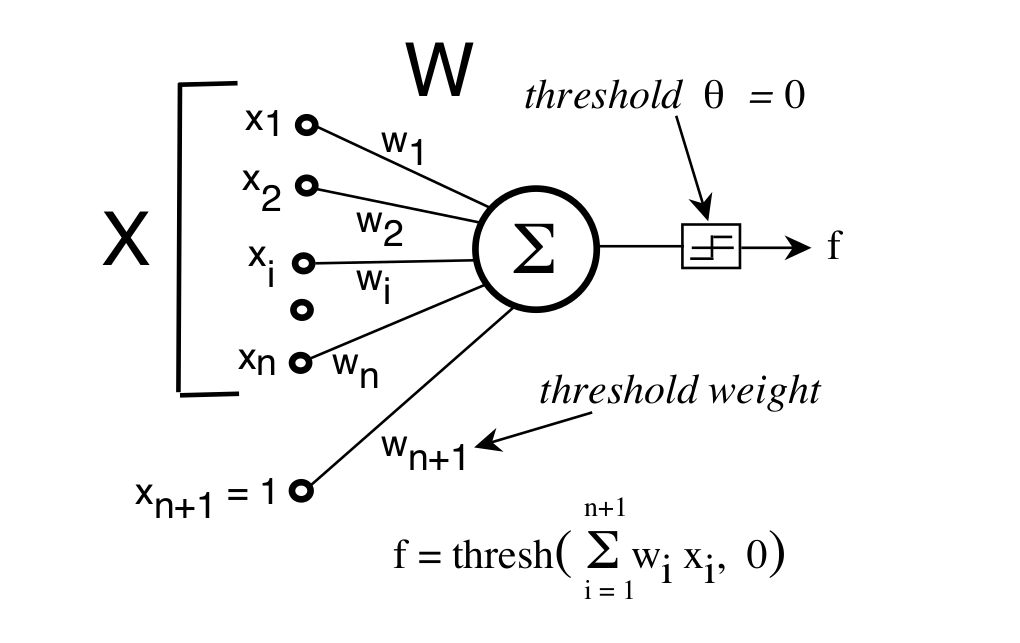
\includegraphics[width=0.70\textwidth]{figs/schema_neurone.png}
	\caption{Illustrazione della struttura di un neurone (~\cite{Intro_retiN}).}
	\label{schema_neurone}	
\end{figure} \\
Quindi il neurone opera la seguente somma pesata:
\begin{equation}
	s_k = \textbf{x}\bullet\textbf{w}_\textbf{k} = \sum_{i=1}^{m}x_iw_{ki}
	\label{sk}
\end{equation}
e si ottiene l'output attraverso la funzione di attivazione: 
\begin{equation}
y_k = \phi(s_k + b_k)
\end{equation}
Risulta utile spendere qualche parola in più sul tipo di funzione di attivazione più utilizzata, ovvero la funzione sigmoide:
\begin{equation}
	sig(x) = \frac{1}{1 + e^{-{\alpha}x}}
\end{equation} 
dove $\alpha$ è un parametro che permette di regolare la pendenza della curva, come si evince dalla figura ~\ref{sigmoide}
\begin{figure}[h!]
	\centering
	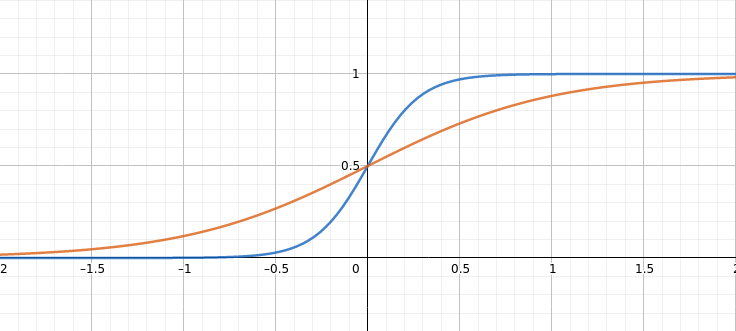
\includegraphics[width=0.75\textwidth]{figs/sigmoide.png}
	\caption{Si riportano due sigmoidi, dove per quella in rosso si ha $\alpha$=2 e per quella in blu $\alpha$=7.}
	\label{sigmoide}
\end{figure}
\newpage
Un singolo neurone è l'ingrediente fondamentale di una rete neurale e nella gran parte dei casi non è in grado di svolgere da solo nessun compito interessante ma deve sempre essere inserito in una rete. Tuttavia esiste una caso particolare nel quale un singolo neurone può portare a termine un compito di classificazione; affinché ciò sia possibile è necessario che i vettori evento siano riconducibili a due sole categorie e che il loro spazio possa essere separato (in relazione alle due categorie) da un singolo iper-piano. In questo caso esiste un teorema di convergenza che garantisce appunto la convergenza dei pesi nel processo di addestramento.

A questo punto è possibile passare ad un livello di complessità superiore, osservando in che modo possono essere organizzati i neuroni per formare la rete neurale; si distinguono due tipologie di reti:
\begin{enumerate}
	\item Reti feedforward con uno o più strati: in questo caso il segnale si propaga dai nodi di input verso quelli di output, senza connessioni fra i neuroni di uno stesso strato;
	\item Reti feedback: sono reti cicliche dove il segnale si propaga anche fra i neuroni di uno stesso strato.
\end{enumerate}
Bisogna chiedersi ora in che modo apprende il singolo neurone. Una delle possibilità (nel caso in cui sia noto l'output target) è l'apprendimento con correzione di errore, che viene presentato velocemente nel seguito.
Si consideri un singolo neurone che ha in ingresso una serie di input $(x_1,...,x_n)$ e quindi produce un valore di output $y$ attraverso la somma pesata già introdotta precedentemente; tale valore può quindi essere confrontata con il risultato atteso $R$, ottenendo così un errore $err = R - y$; si può quindi definire la funzione di costo
\begin{equation}
	E = \frac{1}{2}err^2
\end{equation}
sulla quale si applicherà il metodo di discesa del gradiente già discusso nel paragrafo $2.1$ per ottimizzare i parametri.\\
Una volta capito in che modo avviene l'addestramento di un singolo neurone, è possibile trattare le diverse funzioni che può svolgere una rete neurale:
\begin{enumerate}
	\item L'associazione, a sua volta divisibile in autoassociazione ed eteroassociazione. Nel primo caso vengono presentati alla rete neurale una serie di vettori evento nella fase di training per poi verificare se uno di questi vettori, ripresentato parzialmente, viene nuovamente riconosciuto dalla rete e completato (tale funzione ben si presta ad essere ottenuta a seguito di un processo di apprendimento non supervisionato); nel secondo caso si utilizza un vettore non ancora noto alla rete neurale come richiamo di una già processato;
	\item Il riconoscimento consiste nell'associazione da parte della rete di un vettore evento ad una delle varie categorie possibili. Tale obiettivo può essere ottenuto a seguito di una fase di addestramento dove vengono forniti alla rete sia i vettori in input che le categorie alle quali questi appartengono (si tratta chiaramente di un processo di apprendimento non supervisionato). Si ipotizzi di avere a disposizione dei vettori evento con un numero n di componenti (i dati) e, chiaramente, possono essere pensati come dei punti in uno spazio n-dimensionale; questo spazio potrà essere allora diviso in delle regioni che corrispondono alle varie categorie di cui si è parlato precedentemente ed i confini di queste zone si ottengono a seguito del processo di addestramento;
	\item L'approssimazione di funzioni, dove si hanno a disposizione gli input $\textbf{x}_\textbf{i}$ ed i corrispettivi output $\textbf{y}_\textbf{i}$. Quello che si cerca di fare è approssimare al meglio la funzione $\textbf{y} = f(\textbf{x})$ vera con una $g(\textbf{x})$, tale per cui la distanza euclidea è inferiore ad un valore prefissato positivo (piccolo) $\epsilon$:
		\begin{equation}
			\Vert g(\textbf{x}) - f(\textbf{x}) \Vert < \epsilon
		\end{equation}
\end{enumerate}

Arrivati a questo punto è possibile esporre la trattazione su come una rete neurale viene addestrata. Precedentemente si è introdotta la struttura di una rete neurale, specificando le differenze fra lo strato di input, quello di output e gli strati nascosti. Ogni singolo neurone nel suo processo di addestramento deve aggiornare i suoi pesi, in modo che l'output della rete neurale sia simile a quello atteso.\\
Uno dei metodi migliori per addestrare la rete neurale è l'algoritmo di back-propagation. \\
Una rete neurale è caratterizzata da due tipologie di segnale: da un lato vi è un segnale di funzione che si propaga dallo strato di input verso quello di output e, dall'altro, vi è un segnale di errore che ha origine nello strato di output e si propaga verso quello di input. E' il segnale di errore a giocare un ruolo fondamentale nel processo di apprendimento tramite ottimizzazione dei pesi che caratterizzano la rete neurale. \\
Addentrandosi nell'algoritmo di back-propagation bisogna fare una distinzione fra il modo in cui esso viene applicato allo strato di output ed il modo in cui viene applicato agli strati nascosti:
\begin{enumerate}
	\item Neurone nello strato di output.\\
	Si consideri uno strato di output con un numero n di neuroni e ci si focalizzi sul k-esimo. In un certo momento del processo di apprendimento, alla rete neurale si starà presentando il j-esimo elemento del training data set, quindi per il neurone k si otterrà il seguente segnale di errore:
	\begin{equation}
		err_k^{(j)} = R_k^{(j)} - y_k^{(j)}
	\end{equation}
	dove con la lettera y si intende il valore ottenuto in output dal neurone e con R il valore atteso. \\
	L'errore totale dello strato di output per il vettore evento j-esimo viene definito nel seguente modo:
	\begin{equation}
		E^{(j)} = \frac{1}{2} \sum_{k=1}^{n} (err_k^{(j)})^2
	\end{equation}
	Se poi N è il numero totale di elementi del training data set, allora la funzione di costo può essere definita nel seguente modo:
	\begin{equation}
	E_{tot} = \frac{1}{N}\sum_{j=1}^{N} E^{(j)}
	\end{equation}
	e l'obiettivo è quello di minimizzare tale funzione di costo. Per fare ciò si procede aggiustando i pesi a seguito della presentazione di ogni singolo vettore evento.
	Si utilizza il metodo di discesa del gradiente, procedendo nel seguente modo: \\
	il gradiente è dato da
	\begin{equation}
		\frac{\partial E^{(j)} }{\partial w_{ki}^{(j)}}
	\end{equation}
	e gli aggiornamenti del peso vengono applicati nel verso opposto del gradiente, ovvero
	\begin{equation}
		\Delta w_{ki}^{(j)} = -\mu \frac{\partial E^{(j)} }{\partial w_{ki}^{(j)}}
	\end{equation}
	con $\mu$ fattore di apprendimento.
	Manca a questo punto il calcolo esplicito del gradiente, che può essere eseguito con la regola della catena 
	\begin{equation}
		\frac{\partial E^{(j)} }{\partial w_{ki}^{(j)}} = \frac{\partial E^{(j)}}{\partial err_k^{(j)}}
		\frac{\partial err_k^{(j)}}{\partial y_k^{(j)}}
		\frac{\partial y_k^{(j)}}{\partial S_k^{(j)}}
		\frac{\partial S_k^{(j)}}{\partial w_{ki}^{(j)}}
	\end{equation}
	dove $S_k^{(j)} = s_k^{(j)} + b_k^{(j)} $ (si faccia riferimento all'equazione \eqref{sk}). \\
	Una volta calcolate le quattro derivate si ottiene:
	\begin{equation}
		\frac{\partial E^{(j)} }{\partial w_{ki}^{(j)}} =
		-err_k^{(j)}\phi'(S_k^{(j)})y_i^{(j)}
	\end{equation}
	 e quindi:
	 \begin{equation}
	 	\Delta w_{ki}^{(j)} = err_k^{(j)}\phi'(S_k^{(j)})y_i^{(j)} \mu
	 \end{equation}
	
	\item Neurone in uno strato nascosto \\
	In questo caso l'output del neurone non ha un diretto valore con il quale può essere confrontato, quindi il segnale di errore deve essere determinato a partire dai segnali di errore di tutti i neuroni dello strato successivo, da cui il nome di back-propagation proprio perché il segnale di errore prosegue all'indietro dall'output verso l'input.
\end{enumerate}
Come ultima considerazione sulle reti neurali bisogna sottolineare che il coefficiente di apprendimento deve essere scelto in maniera accurata, infatti se fosse troppo piccolo si avrebbe una convergenza estremamente lenta e, viceversa, un valore troppo grande porterebbe ad una instabilità con comportamento oscillatorio.

\newpage

\subsection{Alberi Decisionali}
\label{alberi decisionali}

Un problema di classificazione può essere sempre trattato in forma di albero decisionale;
applicazioni in sequenza di una serie di test, fatti sugli attributi
l'albero decisionale non è altro che una funzione che a partire dal vettore di input, le cui componenti in questo caso le chiamo attributi, a seguito di una sequenza di test restituisce un singolo valore di output

gli attributi in input possono essere sia continui che discreti (caso più semplice)

output a due valori -> classificatore booleano (o si o no, o segnale o fondo)

differenza tra nodo interno, dove avviene il test sul valore di uno degli attributi e gli archi che ne dipartono corrispondono ai possibili valori e nodo foglia (terminale) che mi dà il possibile risultato finale del processo decisionale

come posso capire a partire dall'abbinamento fra vettore degli attributi e output l'ordine con il quale avvengono i test?
Si vanno a cercare di volta in volta i criteri più discriminanti -> servirà un algoritmo riorsivo